\documentclass[12pt,a4paper]{article}
\usepackage[utf8]{inputenc}
\usepackage[left=20mm,top=20mm,bottom=30mm]{geometry}
\usepackage{graphicx}
\usepackage{alltt}
\usepackage{color, colortbl}

\definecolor{lightgray}{gray}{0.9}
\definecolor{darkgray}{gray}{0.8}

\newcommand{\tab}{\hspace*{2em}}

\begin{document}
\title{Prosjektplan \\ for \\ SkyHiGH Feide}
\author{Fredrik Magnussen, Håkon Tvedt og Morten Hanssen Singstad}
\maketitle
\begin{center}
	
\includegraphics[scale=1]{logo.png}
\end{center}

\newpage
\tableofcontents

\newpage
\section{Mål og rammer}
\subsection{Bakgrunn}
\subsection{Prosjektmål (Effektmål og resultater)}

\section{Omfang}
\subsection{Oppgavebeskrivelse}
\subsection{Avgrensning}

\section{Prosjektorganisering}
\subsection{Ansvarsforhold og roller}
\subsection{Rutiner og regler i gruppen}
\subsection{Verktøy}

\section{Planlegging, oppfølging og rapportering}
\subsection{Hovedinndelinger av prosjektet}
Første del av prosjektet, vil gå til å lese gjennom de foregående SkyHiGH-prosjektene, for å kunne forstå hva som er 
gjort tidligere. Med dette får vi vite enda mer hvordan vi skal sette opp igjen skyløsningen for VM-er med Openstack.
Openstack har også kommet med en ny oppdatering, derfor må vi også finne ut om vi må gjøre endringer, med tanke på installeringen 
av SkyHiGH Adm-delene. Siden vi foreløpig må vente på strøm og Internett til serverne som vi skal bruke, så blir vi nødt til å mongo
sette opp og teste Openstack med SkyHiGH Adm på en VM, på vår egen maskin. \newline \newline
Med dette så kan vi få begynt på del to. Siden vi er driftere så vil vi følge en uskreven regel som sier; Kan en oppgave automatiseres, så skal den automatisere.
Med dette så skal vi lage script. Script for installering av OS på serverne. Script for å ta backup som et image av OS-et, med de siste konfigurasjonene og installeringer.
Dette er også for at det skal spare oss for problemer. Hvis vi skulle være så uheldige med f.eks systemet vårt, så vil vi alltid ha en fungerende installasjon, uten å miste
altfor mye arbeid. Ikke bare vil dette gagne oss, men det er en "best practise" med tanke på at hvis systemet skulle bli gå dukken på grunn av andre hendelser. Da vil 
man kunne få systemet opp å gå på veldig kort tid. \newline \newline
Når vi får gjort oss ferdig med dette, så skal vi parallelt ha jobbet med å få opp strøm og nettverk til der serverne står. Da er vi klare
til å sette rack-et med installasjoner. Til dette bruker vi installerings-scriptet. 

\subsection{Plan/krav for statusmøter og beslutningspunkter}
Ved at vi bruker Scrum som utviklingsmodell så blir planleggingen gjort utifra den. 
\begin{description}
	\item[\tab  •] Product backlog, Sprint backlog, Sprint, Dagsmøter, Sprintmøter og deretter Ferdig modul.
\end{description}
\textbf{Product backlog:}
\tab Slutt produktet som er bestilt av arbeidsgiver deles opp i “stories” som vil tilsvare “product backlog”-moduler. Disse er utarbeidet i henhold til møter med arbeidsgiver, angående hvordan sluttproduktet skal fungere og hvilke krav for brukergrensesnitt det skal være. \newline
\textbf{Sprint backlog:}
“Product backlog story” blir delt opp i mindre arbeidsoppgaver som kan fordeles utover sprint-en og dagsarbeid.
Sprint: En sprint har vi satt til å være en uke. Her jobber vi med sprint backloggen og det forventes å ha ferdig modul innen endt sprint. \newline
\textbf{Dagsmøter:}
Her diskuteres hva som er gjort, hva som skal gjøres og arbeidsfordeling. Skal ikke overskride 30 minutter. \newline
\textbf{Sprintmøte:}
Møte inneholder scrumleder/veileder, arbeidsgiver og scrumteam. Status på “product backlog”-modulen. Legger fram det som er gjort for arbeidsgiver og tar imot kritikk og forslag til endringer. Hvis modulen er ferdig, vis en demo og presenter hvilken ny “product backlog story” skal vi jobbe med. Hvis modulen ikke er ferdig trengs det en ny sprint på foregående modul.

\subsection{Ressursbehov}
Siden produktet blir satt i produksjon, så trenger vi et oppsett som kan fungere og vare en stund. Med dette vil ressursbehovet være 8 servere. 1 til controller- og network node, 5 til compute noder, 2 til lagring og 1 switch. Og siden vi ikke har full tilgang til utstyret, trenger vi også en KVM-console og KVM-switch.

\section{Organisering og kvalitetssikring}
For at vi skal få et best mulig produkt. Så må vi ha en god plan for hvordan vi skal jobbe, vi setter oss standarder for hvordan og når vi gjør dokumentasjoner, rapporter, typologi og kodesyntax.

\subsection{Dokumentasjon, standardbruk og kildekode}
Rapportskriving av arbeid vil skje løpende og vil hjelpe med å kunne forsklare kunden hva vi har gjort og hvordan. \newline \newline
Dokumentasjon ligger under det samme, men dette må et mye grundigere nivå. Her er det snakk om dokumentering med en samling av kodelinjer, dokumentere funn, løsninger og hvordan vi bruker forskjellige oppsett. Dette gjør vi for at vi ikke skal bruke unødvendig krefter på tid og frustrasjon ved å forstå hva de andre på gruppen har gjort, samt hva vi selv gjorde for lenge siden. \newline \newline
Siden vi bruker Openstack som kjører på Apache 2.0 lisens så følger vi standarder til Apache 2.0.


\newpage
\subsection{Risikoanalyse}
\begin{table}[h]
	\begin{tabular}[Figur 1]{| p{3cm} | p{3cm} | p{5cm} | p{5cm} |}
		\hline \rowcolor{lightgray} \textbf{Beskrivelse} & \textbf{Sannsynlighet} & \textbf{Konsekvens} & \textbf{Løsning} \\
		\hline \rowcolor{darkgray} Sykdom blant teamet & lav & Mangel på arbeidskraft & Tilrettelegging av arbeidsforhold for den syke. \\
		\hline \rowcolor{lightgray} Tap av data ved tekniske feil eller menneskefeil (skrive over eller sletter feil). &	lav/middels &	Detter langt tilbake i arbeid og kan resultere i at  oppgaven blir veldig redusert. Mye ekstra jobb. & Kontinuerlig backup(automatisert) og repository på det vi skriver. \\
		\hline \rowcolor{darkgray} Mangel på kompetanse &	middels & Bruker lengre tid på å få til, rekker ikke tidsfrister og kan resultere i dårlig utførelser. & Les seg opp, samarbeide for å forstå. Få  informasjon fra noen med kompetanse. \\
		\hline \rowcolor{lightgray} Dårlig tidsplanlegging & høy & Mer jobb en det vi trodde. Sluttprodukt kan risikere å ikke bli ferdig. & Ikke undervurdere mengde arbeid. \\
		\hline \rowcolor{darkgray} Endringer som er ødeleggende &	middels/høy	 & Tap av data, konfigurasjon og oppsett. & Backup, automatisert installasjon, mulighet for rollback. \\
		\hline \rowcolor{lightgray} Dårlig dokumentering & lav/middels & Vanskelig å rette opp feil. Hvis systemet må settes opp på nytt, er dokumentering viktig for å se hva vi har gjort. & Passe på hverandre i forhold til dokumentasjon. Ofte påminning.
	\end{tabular}
\end{table}


\section{Plan for Gjennomføring}
\subsection{Fremdriftsplan}

\section{Prosjektavtale}

\section{Referanser}

\newpage
\section{Grupperegler}
\begin{flushright}
	\begin{figure}[h]
		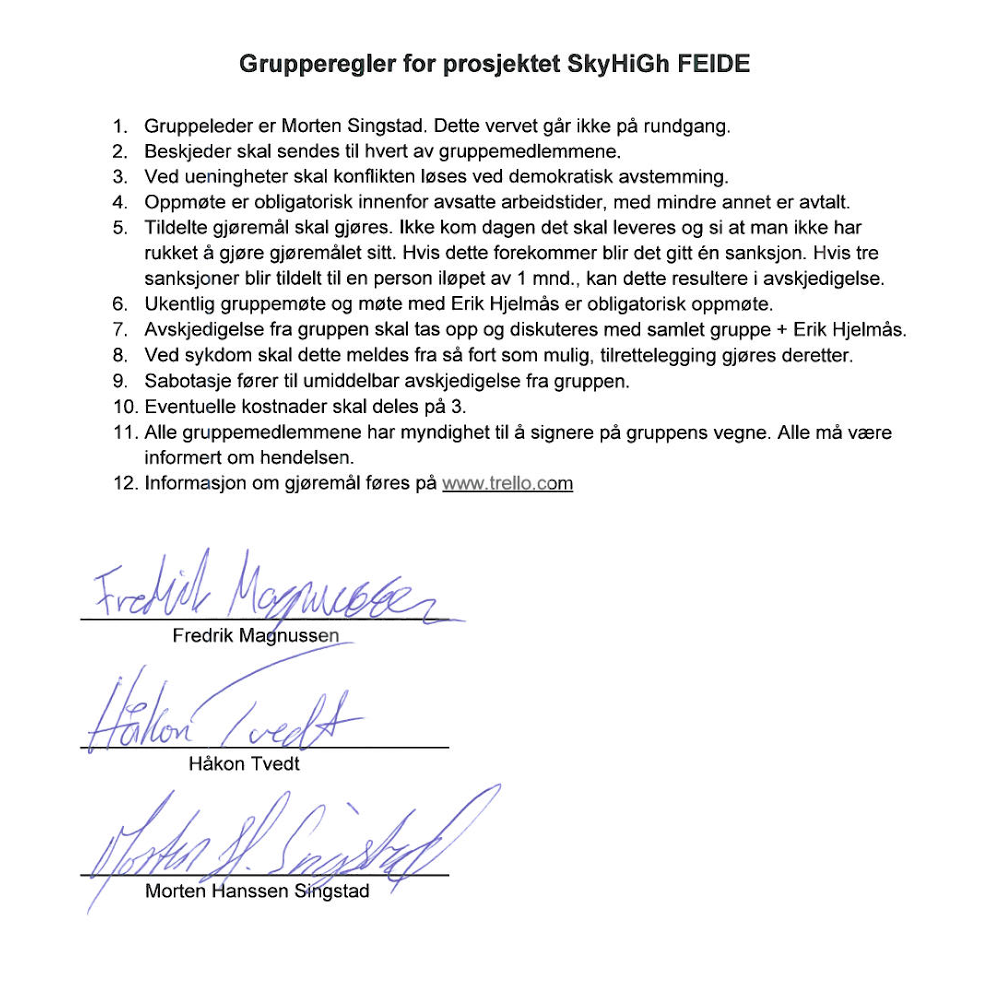
\includegraphics[width=150mm,height=150mm]{grupperegler.png}
 	\end{figure}
\end{flushright}

\end{document}
